\section{Desarrollo / Análisis de Resultados}
\subsection{Análisis de SW}
\begin{figure}[H]
    \centering
    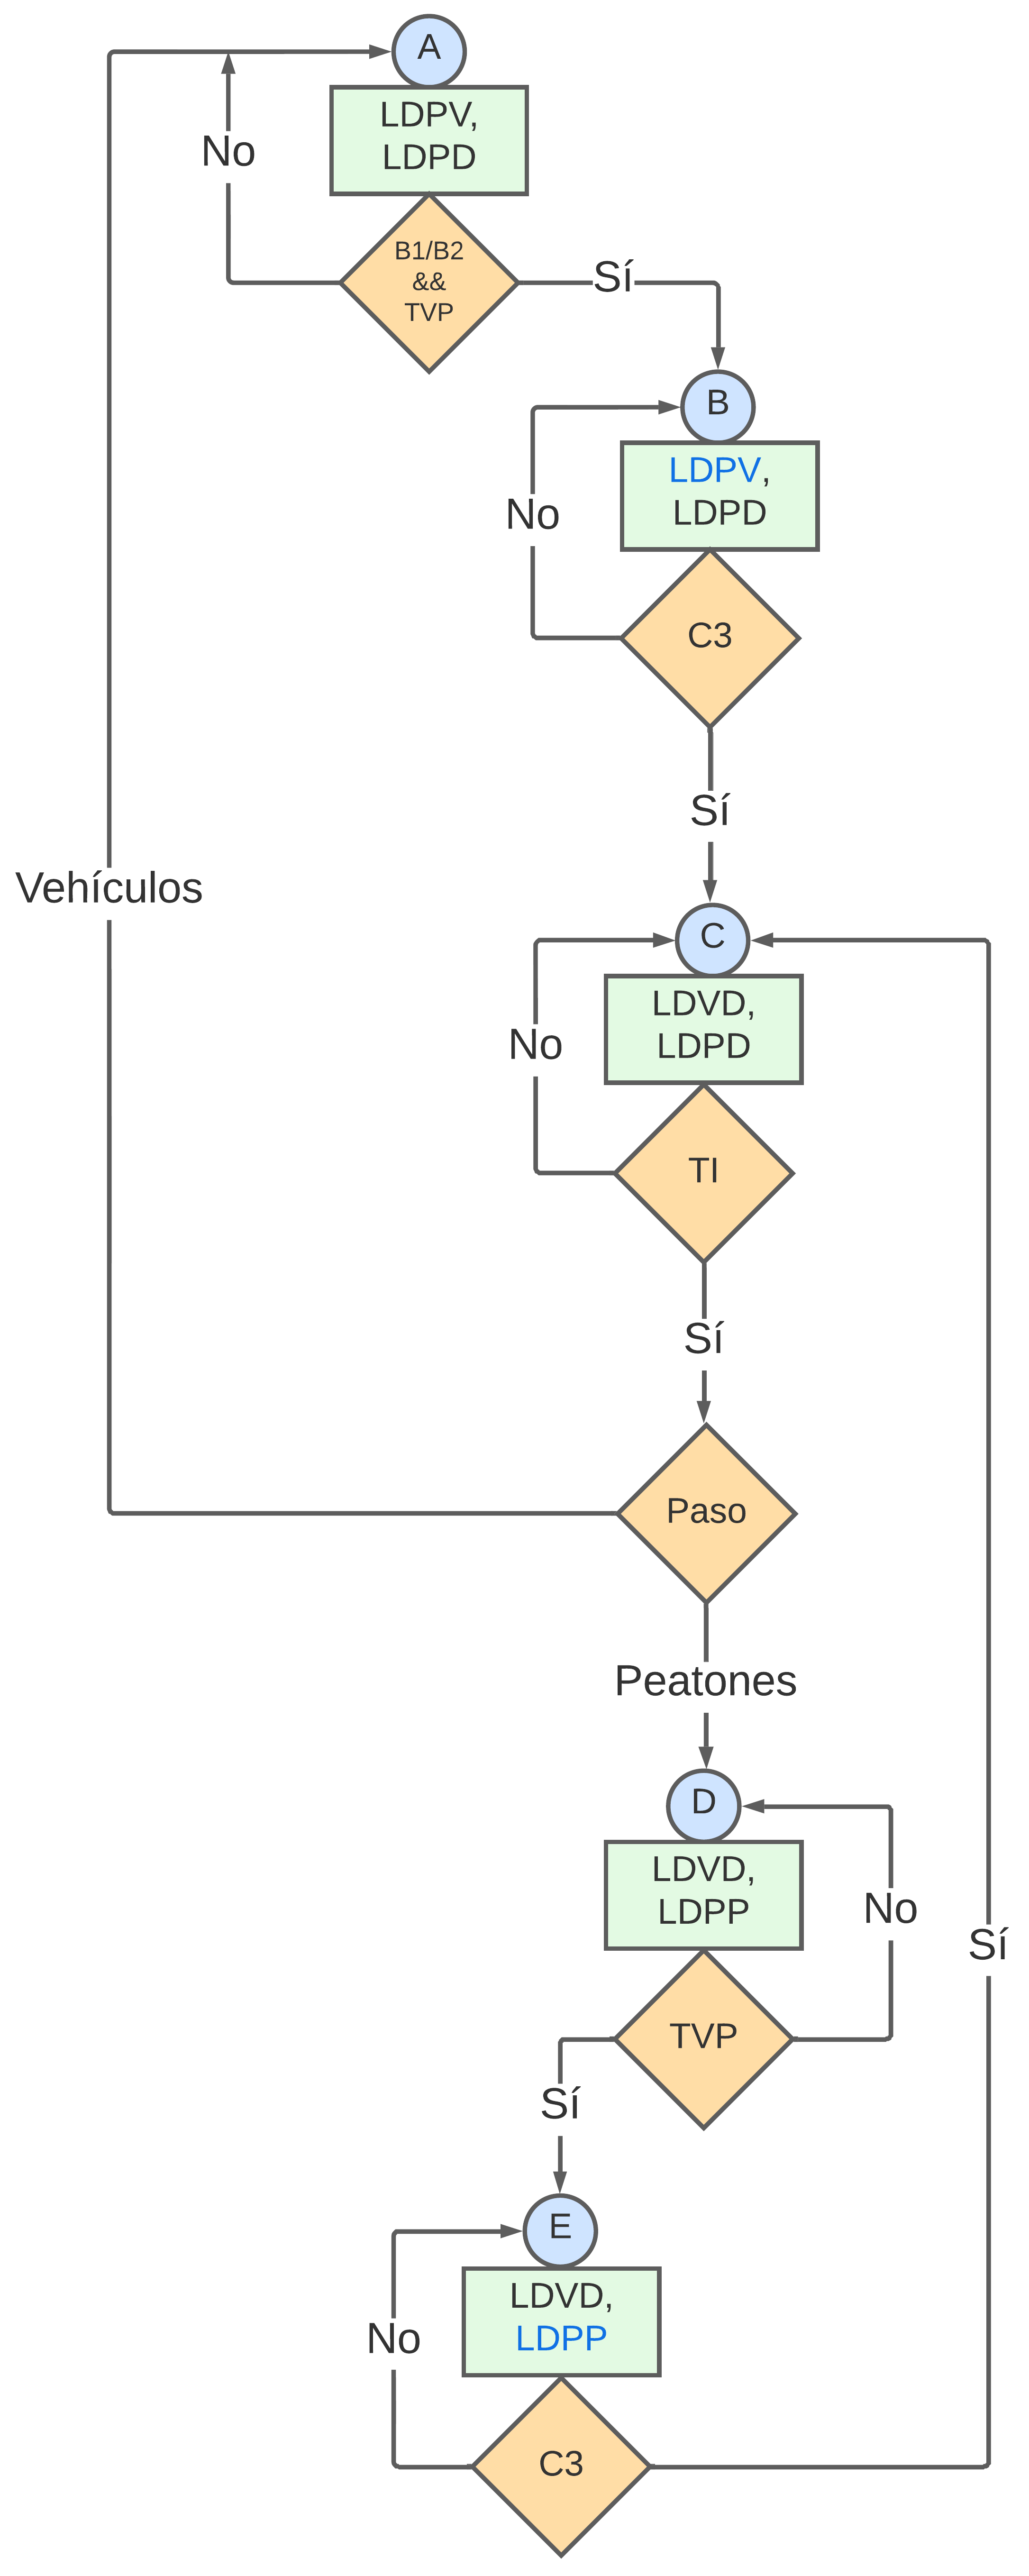
\includegraphics[width=0.45\textwidth]{images/diagrama_asm.png}
    \caption{Diagrama ASM propuesto para el cruce de semáforos. Creación propia}
    \label{diagrama_asm}
\end{figure}

En la figura \ref{diagrama_asm} se puede observar el diagrama ASM construido para el cruce de semáforos mostrado en la figura \ref{cruce_semaforos}. En la siguiente tabla se presenta la descripción de la nomenclatura empleada en el diseño del diagrama: 

\begin{table}[H]
\centering
\renewcommand{\arraystretch}{1.25}
\begin{tabular}{|c|c|c|}
\hline
\multirow{5}{*}{Entradas} & B1   & Botón de semáforo peatonal 1                            \\ \cline{2-3} 
                          & B2   & Botón de semáforo peatonal 2                            \\ \cline{2-3} 
                          & TVP  & Timer de paso de vehículos o peatones (10 segundos)     \\ \cline{2-3} 
                          & TI   & Timer de 1 segundo                                      \\ \cline{2-3} 
                          & C3   & Contador de parpadeos (cuenta hasta 3 segundos)         \\ \hline
\multirow{4}{*}{Salidas}  & LDPV & Led de paso de vehículos                                \\ \cline{2-3} 
                          & LDPD & Led de peatones detenidos                               \\ \cline{2-3} 
                          & LDVD & Led de vehículos detenidos                              \\ \cline{2-3} 
                          & LDPP & Led de paso de peatones                                 \\ \hline
\multirow{5}{*}{Estados}  & A    & Paso de vehículos por al menos 10 segundos              \\ \cline{2-3} 
                          & B    & Parpadeo de luz verde del semáforo vehicular (LDPV)     \\ \cline{2-3} 
                          & C    & Paro total de vehículos y peatones por 1 segundo        \\ \cline{2-3} 
                          & D    & Paso de peatones por 10 segundos                        \\ \cline{2-3} 
                          & E    & Parpadeo de luces verdes de semáforos peatonales (LDPP) \\ \hline
\end{tabular}
\caption{Entradas, salidas y estados del diagrama ASM propuesto. Creación propia}
\renewcommand{\arraystretch}{1}
\end{table}

En programación orientada a objetos, una máquina de estados podría considerarse como una clase con una colección de variables de estado y métodos que activan las salidas correspondientes a cada estado. Sin embargo, en C no se tiene la posibilidad de escribir clases, ya que este es un lenguaje es procedimental. No obstante, hay formas de simular mecanismos propios de la programación orientada a objetos en C. En esta caso para imitar una clase se utilizó un \textit{struct}, una estructura especial de C, en la cual se definieron los miembros que componen cada estado de la máquina:

\begin{minted}{C}
typedef struct Semaforo{
  void (*state_func_ptr)(void);
  int time;
} FSM;
\end{minted}

El puntero \textit{state\_func\_ptr} apunta a la dirección de memoria del microcontrolador en la cual se almacena cada función. Este sirve para hacer los llamados a las funciones correspondientes de cada estado. Por otra parte, el atributo de \textit{time} es un número entero que determina la cantidad de segundos que cada estado debe permanecer activo.

Posteriormente se define la máquina de estados, haciendo un arreglo de 5 \textit{struct FSM}, uno por cada estado:

\begin{minted}{C}
FSM semaforo[5] = {
  {&A_out, 10},
  {&B_out, 3},
  {&C_out, 1},
  {&D_out, 10},
  {&E_out, 3},
};
\end{minted}

Como se puede observar en la porción de código mostrada anteriormente, cada espacio del arreglo \textit{semaforo} contiene un número entero, que representa el argumento \textit{time}. Además, en cada espacio se incluye el nombre de una de las siguientes funciones acompañado con el operador \&, para obtener la dirección en memoria de esa función. \textbf{(Esta mini-fracción de código solo es por comodidad y para fines ilustrativos).}

\begin{minted}{C}
void A_out(void){
  PORTB = 0x09;
}

void B_out(void){
  PORTB ^= 0x01;
}

void C_out(void){
  PORTB = 0x0A;
}

void D_out(void){
  PORTB = 0x06;
}

void E_out(void){
  PORTB ^= 0x04;
}
\end{minted}

Las funciones anteriormente expuestas se encargan de cambiar el estado de los pines del puerto B, según corresponda. Dicho esto, cabe destacar que las funciones \textit{B\_out()} y \textit{E\_out()} invierten el estado de los pines B0 y B2, debido a que estas son las funciones que generan los parpadeos de luces.

Por otro lado, la configuración del timer se encapsuló dentro de la siguiente función:

\begin{minted}{C}
void timer_setup() {
  TCCR0A=0x00; // Modo normal
  TCCR0B=0x00; 
  TCCR0B |= (1<<CS00)|(1<<CS02); // Prescaling de 1024
  sei(); // Se llama a la función sei() para habilitar las interrupciones globales
  TCNT0=0;
  TIMSK|=(1<<TOIE0); // Se habilita la interrupción del timer1
}
\end{minted}

\newpage

Tomando en cuenta que el ATtiny4313 opera con un oscilador interno a $8\,MHz$ y que el prescaling establecido fue de el de 1024, se puede determinar cuantos ciclos del timer se necesitan para contar un segundo de la siguiente forma:

\begin{equation*}
    \text{Frecuencia con prescaling} = \frac{8\,MHz}{1024} = 7812.5 \,Hz
\end{equation*}

\begin{equation*}
    \text{Periodo con prescaling} = \frac{1}{7812.5 \,Hz} = 0.128\,ms 
\end{equation*}

Para terminar una cuenta del timer se necesitan entonces:

\begin{equation*}
    255 \cdot 0.128\,ms = 0.03264\,s
\end{equation*}

Por lo tanto, para contar un segundo se necesitan:

\begin{equation*}
    \frac{1\,s}{0.03264\,s} \approx \text{31 ciclos}
\end{equation*}

Cabe mencionar que el resultado anterior se bajó a $30\,s$ por comodidad.

Más adelante, se configuró el Interrupt service routine de la siguiente forma, para que únicamente cambiara el estado de una variable \textit{B1\_B2}, utilizada para guardar la solicitud de paso peatonal:

\begin{minted}{C}
ISR (INT1_vect) {     
  B1_B2 = 1;
}
\end{minted}

Por otro lado, el Interrupt vector para el Timer0 se configuró de la siguiente forma:

\begin{minted}{C}
ISR (TIMER0_OVF_vect){
  if((int_count) == 1 || (int_count == 15)){ // Cuenta de medio segundo
    if(state == B){
      (semaforo[B].state_func_ptr)(); // Llamado a salidas de estado B
    }
    if(state == E){
      (semaforo[E].state_func_ptr)(); // Llamado a salidas de estado B
    }
  }
  else if(int_count == 30){ // cuenta de un segundo
    ++TI;
    int_count = 0;
  }
  if(TI == 10){
    ++TVP;
  }
  ++int_count;
}
\end{minted}

Aquí se puede observar que hizo uso de la cuenta de 30 ciclos por segundo para determinar el aumento de las variables de temporización \textit{TI},\textit{TVP} y \textit{int\_count}. La última de estas aumenta con cada ciclo y, por lo tanto, al llegar a 30 cuenta un segundo. Asimismo, es en esta parte que se llama a las funciones \textit{B\_out()} y \textit{E\_out()}, las cuales se encargan de hacer que las luces parpadeen. Ambas se llaman cada medio segundo durante un total de 3 segundos.

Finalmente, en la función \textit{main()} primeramente se hacen las configuraciones necesarias para que el microcontrolador opere de la manera deseada, posteriormente se hace la inicialización de todas las variables y por último se ejecuta un bucle infinito dentro del cual corre la máquina de estados desarrollada.

\begin{minted}{C}
int main(void){
  DDRB = 0x0F; // Configurando los pines de entrada/salida del puerto B
  GIMSK = 0x80; // Habilitando la interrupción externa en INT1  
  MCUCR = 0x08; // Interrupción generada por el flanco decreciente en INT1
  PORTB = 0x00; // Se setean todas las salidas en estado bajo (y se activan las resistencias de pull-up de todas las entradas)
  timer_setup(); // Llamado a configuración del timer

  state = A;
  B1_B2 = 0;
  TVP = 0;
  TI = 0;
  int_count = 0;
  pass_flag = 0;

  while(1){
    switch (state){
      case A:
        .
        .
      case B:
        .
        .
      case C:
        .
        .
      case D:
        .
        .
      case E:
        .
        .
    }
  }
}
\end{minted}

\subsection{Análisis de HW}

El circuito de prueba construido para este proyecto se subdivide en dos secciones importantes: el circuito de control y el de potencia. El primero de estos dos se puede observar en la figura \ref{circuito_control}.

\begin{figure}[H]
\centering
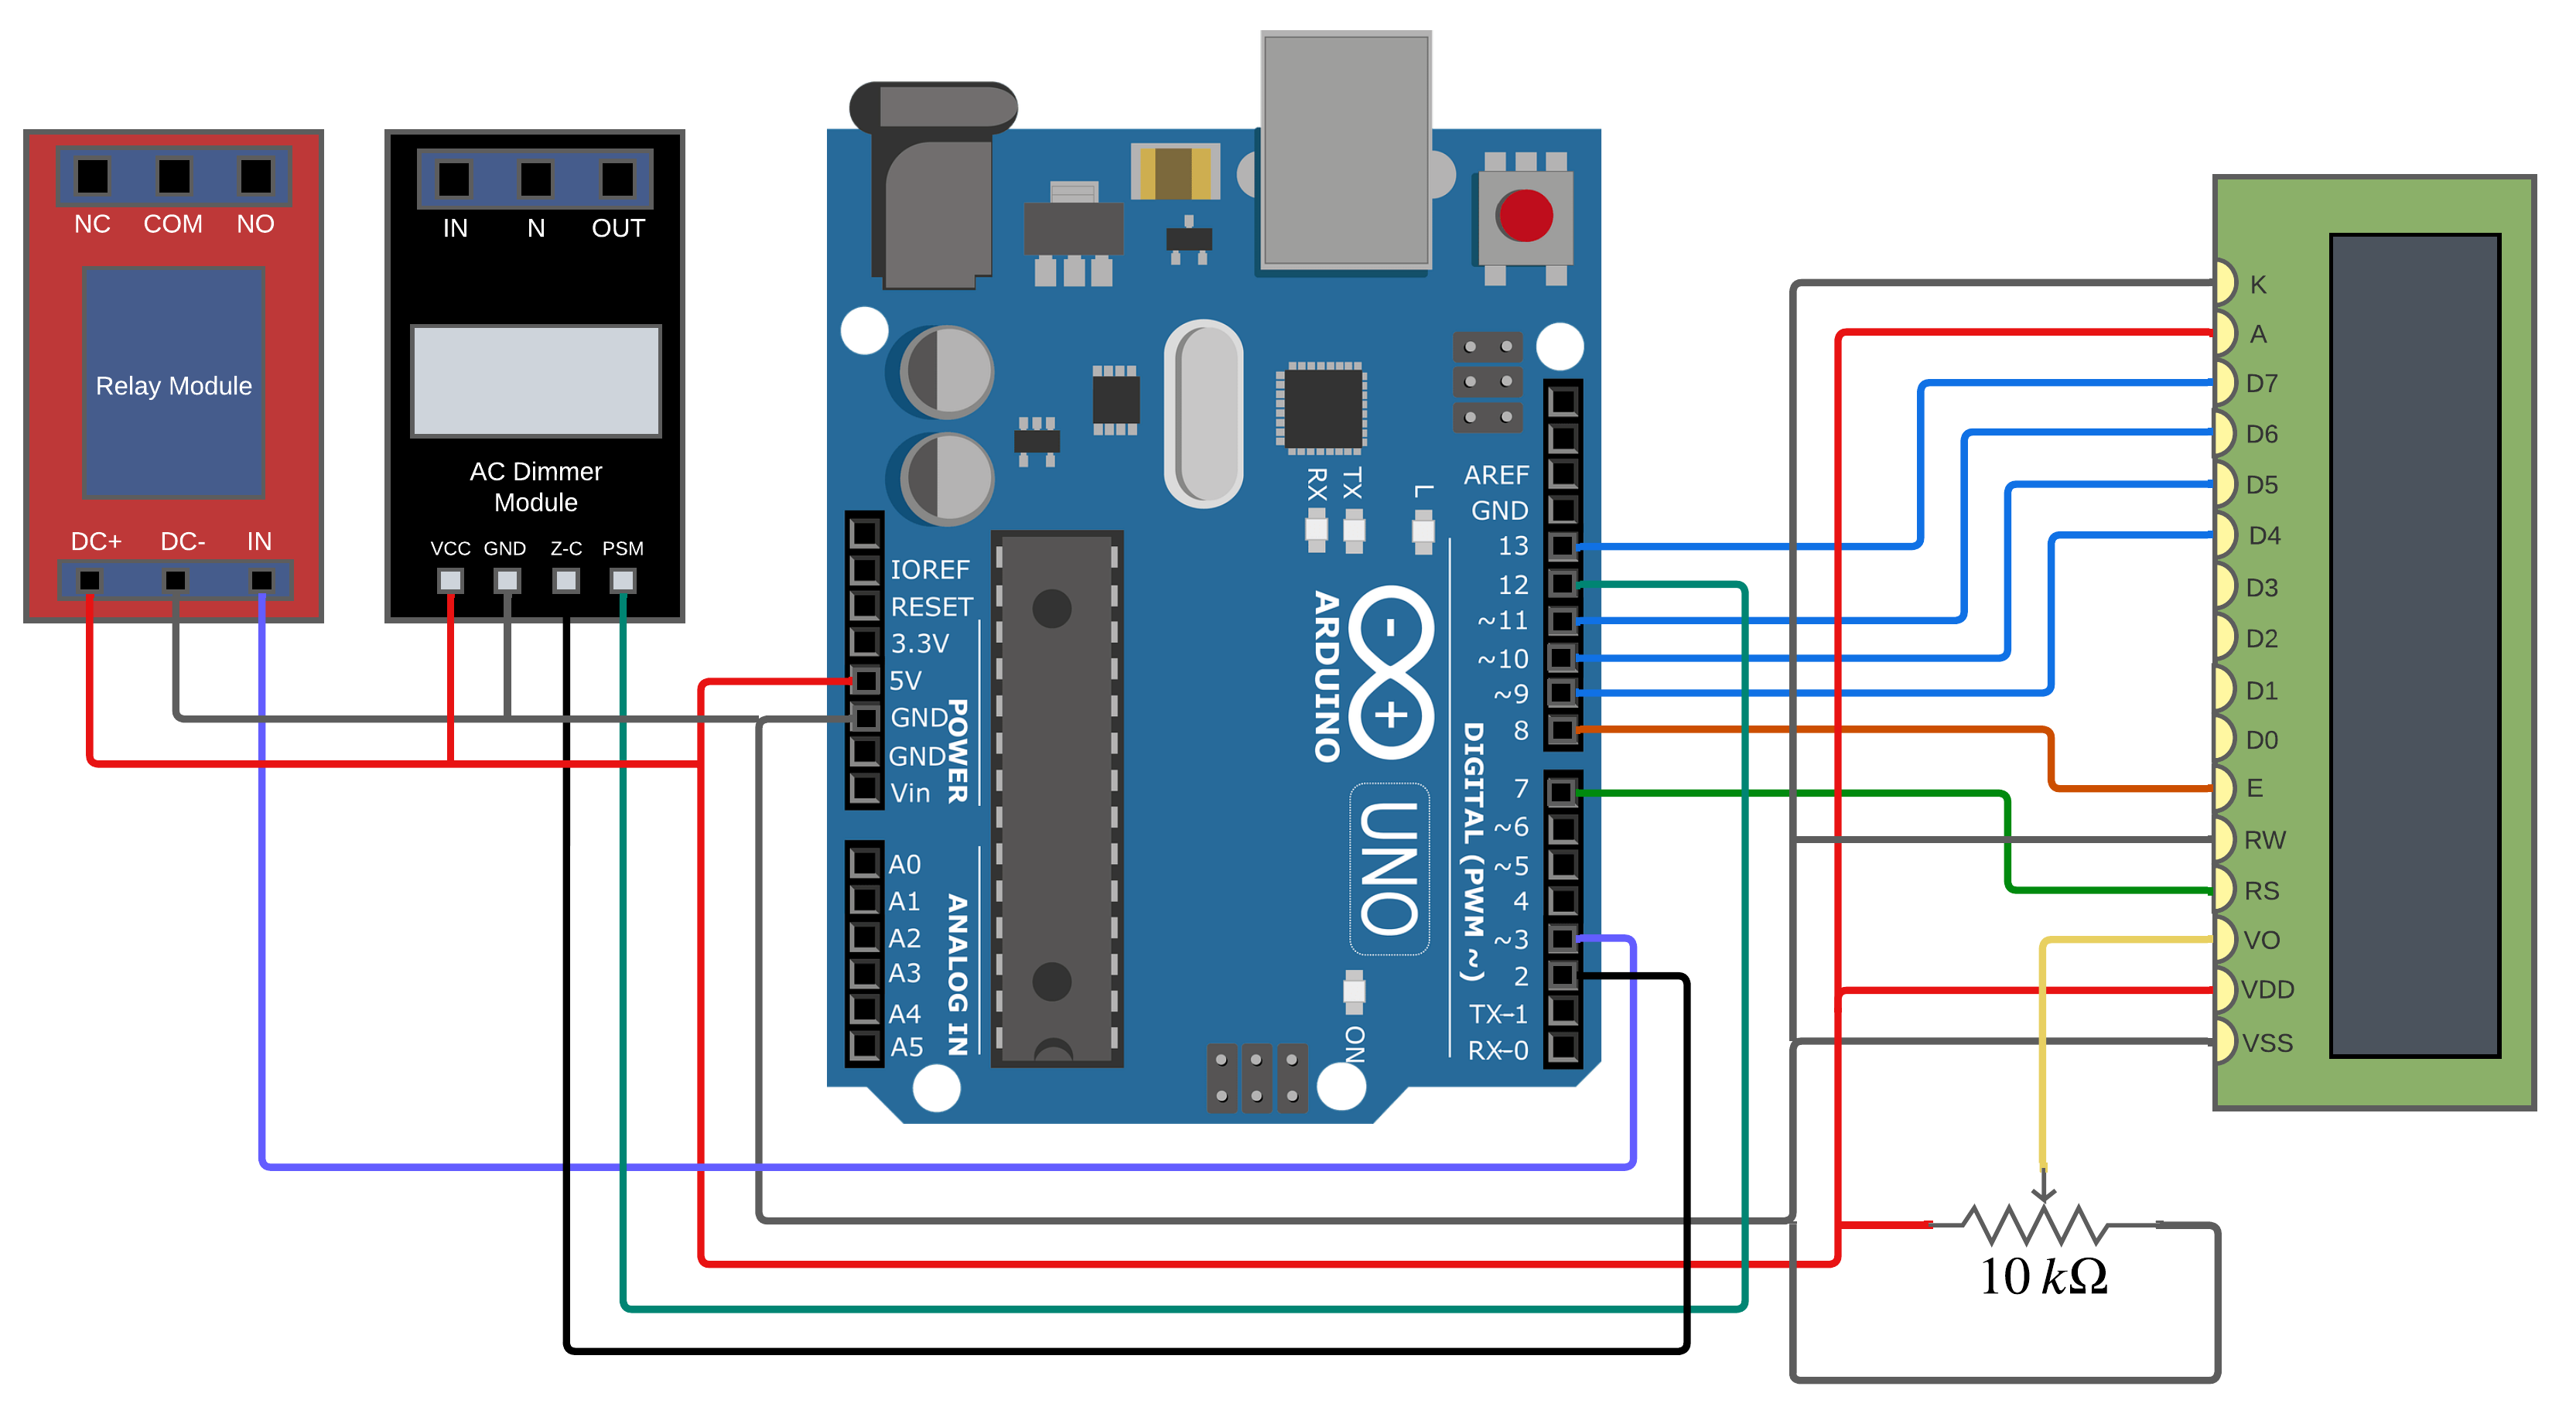
\includegraphics[scale=0.62]{./images/control.png} 
\caption{Diagrama del circuito de control}
\label{circuito_control}
\end{figure}

\vspace*{-0.3cm}

Por otra lado, la parte correspondiente al circuito de potencia se presenta en la figura \ref{potencia}.

\begin{figure}[H]
\centering
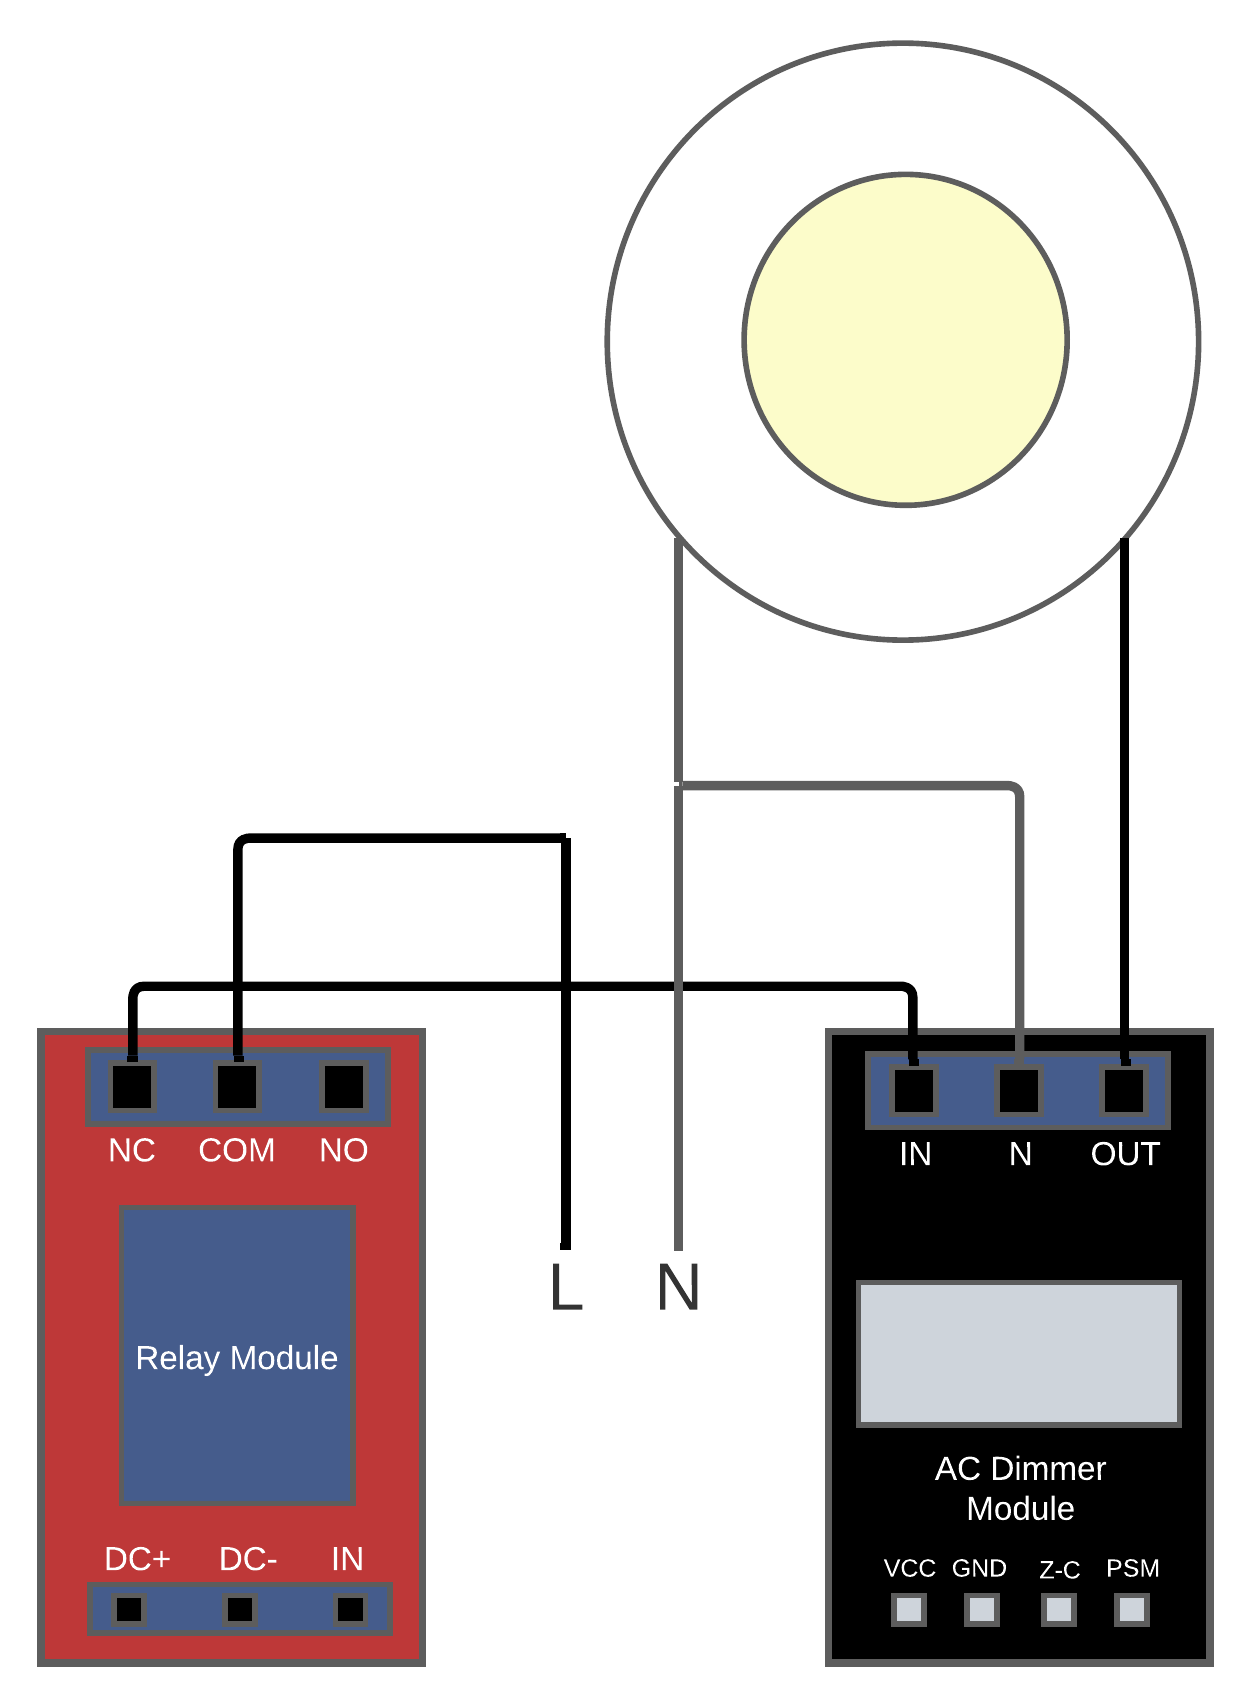
\includegraphics[scale=0.62]{./images/potencia.png} 
\caption{Diagrama del circuito de potencia }
\label{potencia}
\end{figure}

Con respecto al circuito de control, primeramente se sabe que la bobina del relé consume $90\,mA$ y necesita estar alimentada a $5\,V$ para operar correctamente. Al multiplicar estos últimos dos datos se puede determinar que la potencia consumida por el relé es de $450\,mW$. Por otra parte, la pantalla LCD 16x2 presenta un consumo máximo de $25\,mA$ y requiere de $5\,V$ para funcionar, por lo tanto, este componente consume aproximadamente $125\,mW$. En cuanto al módulo dimmer AC, se sabe que sus periféricos pueden operar adecuadamente a cualquier corriente menor a $10\,mA$. Además, este componente también está conectado a la fuente de tensión de $5\,V$ del Arduino UNO. Tomando en cuenta estos datos, se tiene que el módulo dimmer AC puede llegar a consumir hasta $50\,mW$. Al sumar todos los resultados anteriores, se tiene un consumo de potencia de $625\,mA$ por parte del circuito de control. 

Por el lado del circuito de potencia, el único el único elemento que presenta consumo de potencia es la resistencia de la bombilla incandescente. El valor de dicha potencia corresponde a un máximo de $100\,W$.

 \textbf{A continuación se presenta un link para accesar y ver un video de su correcto funcionamiento:}\\



\hspace{0.5mm}\url{https://drive.google.com/drive/folders/12DI6IFieF0CJ9Nj7iPxgw47PLW-znKQv?usp=sharing} 










